\subsection{Parameter estimation of speed distribution}
\label{section_speed_modeling}
In this section, we modeling the speed distribution. we fit the cumulative status average speed distribution to get the cumulative probability distribution function, and then take a derivative with it to obtain the speed probability distribution.

From figure. \ref{figure_fit_ccdf_speed}, the average speed distribution shows exponential law. Given that, we set the function form as follows:

The fit formulas are given as formulas \ref{formular_ccdf_speed}. $f(x)$ is the function form for the average speed distribution of vacant status, and the other one $g(x)$ is for that of occupied status.

\begin{equation}\label{formular_ccdf_speed}
\left\{
\begin{array}{ll}
f(x) = 1-1/exp(a_1x^{1.5})\\
g(x) = 1-1/exp(a_2x^{2.5})
\end{array}
\right.
\end{equation}


Fig. \ref{figure_fit_ccdf_speed} also plots the fit results. 

\begin{figure}
\centering
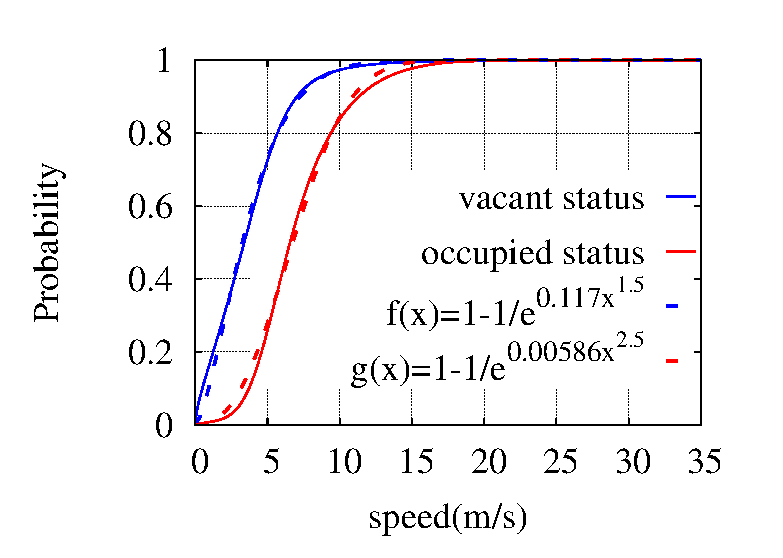
\includegraphics[width=0.4\textwidth]{figures_201103/fit/speedfit.eps}\\
\centering
\caption{The fit result of the cumulative speed distributions.}\label{figure_fit_ccdf_speed}
\end{figure}

The rms of residuals for each fit are as table \ref{table_rms}.The smaller rms of residuals means better fitting. In the table, the values are all less than 0.02, showing good similarity.

\begin{table}
\caption{The parameter and the rms of residuals of fitting curves}\label{table_rms}
\centering
\begin{tabular}{l|c|c}
  \hline
  % after \\: \hline or \cline{col1-col2} \cline{col3-col4} ...
  Categories & rms of residuals  \\
  \hline
  $f(x)$ &$a1=0.117$ &0.0113159\\
  $g(x)$ &$a2=0.0586$ &0.0137029\\
  \hline
\end{tabular}
\end{table}

